
%(BEGIN_QUESTION)
% Copyright 2010, Tony R. Kuphaldt, released under the Creative Commons Attribution License (v 1.0)
% This means you may do almost anything with this work of mine, so long as you give me proper credit

This temperature control system has a problem.  The process temperature is running above setpoint significantly -- the setpoint is 850 $^{o}$F and the temperature (as indicated by TIC-205) is 934 $^{o}$F and showing no signs of cooling off over time:

$$\includegraphics[width=15.5cm]{i01491x01.eps}$$

The operator tells you the process was working just fine yesterday, holding right at the setpoint value of 850 $^{o}$F.  Your first step is to examine the faceplate of the controller: it is in automatic mode, and the output is at a value of $-5$\%.

\vskip 10pt

Explain the rationale behind checking the controller's mode and output value.  How is this information helpful in troubleshooting the problem?  What would be your next step in troubleshooting this problem?  What might you do differently if you had seen the controller in a different mode, or with its output at some different (greater) value?

\vskip 20pt \vbox{\hrule \hbox{\strut \vrule{} {\bf Suggestions for Socratic discussion} \vrule} \hrule}

\begin{itemize}
\item{} How significant is the information that this process was working fine just yesterday?  Would it make any difference to your diagnosis if you had been told this process has never worked right?
\item{} Suppose this system were functioning perfectly well, and then something pinched Cable 3 Pair 2 and caused it to fail shorted.  Explain what would happen as a result of this fault.
\item{} Suppose this system were functioning perfectly well, and then something pinched Cable 3 Pair 1 and caused it to fail shorted.  Explain what would happen as a result of this fault.
\end{itemize}

\underbar{file i01491}
%(END_QUESTION)





%(BEGIN_ANSWER)

The ``automatic'' mode is proper, and the low output signal value tells us the controller is doing all it can to bring the temperature down.  The problem, therefore, is {\it not} in the controller's automatic response!

%(END_ANSWER)





%(BEGIN_NOTES)

Now that we know the controller is not at fault, we may move our investigation to the following areas:

\begin{itemize}
\item{} {\bf Transmitter}: maybe it's reading too high, and the process isn't as hot as the transmitter thinks it is?
\item{} {\bf Controller}: maybe it's misinterpreting the transmitter's signal as being too high, and the process isn't as hot as the controller thinks it is?
\item{} {\bf Final control element}: maybe the valve isn't shutting off like it should for some reason?
\end{itemize}

A good ``next test'' would be to examine the valve stem's position to see whether or not it is indeed fully closed.  Another ``next test'' would be to verify the temperature transmitter's indication of furnace temperature.











\vskip 20pt \vbox{\hrule \hbox{\strut \vrule{} {\bf Virtual Troubleshooting} \vrule} \hrule}

This question is a good candidate for a ``Virtual Troubleshooting'' exercise.  Presenting the diagram to students, you first imagine in your own mind a particular fault in the system.  Then, you present one or more symptoms of that fault (something noticeable by an operator or other user of the system).  Students then propose various diagnostic tests to perform on this system to identify the nature and location of the fault, as though they were technicians trying to troubleshoot the problem.  Your job is to tell them what the result(s) would be for each of the proposed diagnostic tests, documenting those results where all the students can see.

During and after the exercise, it is good to ask students follow-up questions such as:

\begin{itemize}
\item{} What does the result of the last diagnostic test tell you about the fault?
\item{} Suppose the results of the last diagnostic test were different.  What then would that result tell you about the fault?
\item{} Is the last diagnostic test the best one we could do?
\item{} What would be the ideal order of tests, to diagnose the problem in as few steps as possible?
\end{itemize}

%INDEX% Troubleshooting review: electric circuits

%(END_NOTES)


